\documentclass[9pt,twocolumn]{extarticle}
\usepackage[a4paper,margin=1.55cm,columnsep=0.55cm]{geometry}
\usepackage[T1]{fontenc}
\usepackage{lmodern}
\usepackage{mathptmx}
\usepackage{amsmath}
\usepackage{microtype}
\usepackage{graphicx}
\usepackage{booktabs}
\usepackage[numbers,sort&compress]{natbib}
\usepackage[font=footnotesize,labelfont=bf,skip=3pt]{caption}
\usepackage{enumitem}
\usepackage[hidelinks]{hyperref}
\usepackage{titlesec}

\titleformat{\section}{\normalsize\bfseries}{\thesection}{0.5em}{}
\titlespacing*{\section}{0pt}{5pt plus 2pt}{2pt}
\setlist{nosep,leftmargin=*}
\setlength{\bibsep}{0pt}
\setlength{\parskip}{0pt}
\renewcommand{\bibfont}{\scriptsize}

% Generated by `uv run pgnoise numbers` from results/summary.json. Do not edit by hand.
\newcommand{\pgCommit}{144fe22}  % reproduction.proteingym_commit (first 7 characters)
\newcommand{\nModels}{97}  % reproduction.n_models
\newcommand{\nAssays}{217}  % reproduction.n_assays
\newcommand{\nUnits}{200}  % ranks.n_units
\newcommand{\unitsBinding}{12}  % ranks.units_by_group.Binding
\newcommand{\unitsExpression}{18}  % ranks.units_by_group.Expression
\newcommand{\nExactAverage}{97}  % reproduction.columns.Average_Spearman.n_exact_3dp
\newcommand{\nExactRank}{97}  % reproduction.columns.rank.n_exact_3dp
\newcommand{\nExactSE}{91}  % reproduction.columns.Bootstrap_standard_error_Spearman.n_exact_3dp
\newcommand{\nSEOff}{6}  % number of reproduction.se_mismatches
\newcommand{\seOffBoundary}{0.0002}  % max over reproduction.se_mismatches of |ours - nearest 3-dp rounding boundary| (4 dp, rounded up)
\newcommand{\nExactOtherMetrics}{97}  % min over AUC, MCC, NDCG, Top_recall of robustness.reproduction_other_metrics.average_exact
\newcommand{\driftEsmOneV}{0.011}  % version_drift[PG_v1.0].largest_changes, ESM-1v (single), absolute
\newcommand{\driftMaxOneZero}{0.158}  % version_drift[PG_v1.0].max_abs_change
\newcommand{\driftMaxOneTwo}{0.001}  % version_drift[PG_v1.1].max_abs_change
\newcommand{\driftSinceOneTwo}{0.000}  % max of version_drift[from PG_v1.2 on].max_abs_change
\newcommand{\nBoot}{10,000}  % ranks.n_boot
\newcommand{\topOne}{AIDO Protein-RAG}  % ranks.intervals_by_rank.1.model
\newcommand{\topTwo}{VenusREM}  % ranks.intervals_by_rank.2.model
\newcommand{\topThree}{ProSST (K=2048)}  % ranks.intervals_by_rank.3.model
\newcommand{\topFour}{ProSST (K=4096)}  % ranks.intervals_by_rank.4.model
\newcommand{\topTen}{ProSST (K=512)}  % ranks.intervals_by_rank.10.model
\newcommand{\gapOneTwo}{0.00004}  % ranks.gap_1_vs_2
\newcommand{\pRankOneTop}{49}  % ranks.intervals_by_rank.1.p_rank1 (percent)
\newcommand{\pRankOneSecond}{50}  % ranks.intervals_by_rank.2.p_rank1 (percent)
\newcommand{\bestSet}{AIDO Protein-RAG, VenusREM and ProSST (K=4096)}  % ranks.best_set
\newcommand{\nBestSet}{3}  % len(ranks.best_set)
\newcommand{\naiveBestSet}{AIDO Protein-RAG, VenusREM and ProSST (K=2048)}  % ranks.naive_best_set
\newcommand{\nNeighbourSig}{2}  % ranks.neighbours_sig_holm
\newcommand{\nNeighbourSigRaw}{2}  % ranks.neighbours_sig_uncorrected
\newcommand{\zSigA}{4.9}  % ranks.neighbours_sig_z, first pair
\newcommand{\zSigB}{5.9}  % ranks.neighbours_sig_z, second pair
\newcommand{\sigPairA}{VenusREM $>$ ProSST (K=2048)}  % ranks.neighbours_sig_z, first key
\newcommand{\sigPairB}{S3F-MSA $>$ S2F-MSA}  % ranks.neighbours_sig_z, second key
\newcommand{\margFourLo}{1}  % ranks.intervals_by_rank.4.marg_lo
\newcommand{\margFourHi}{13}  % ranks.intervals_by_rank.4.marg_hi
\newcommand{\simFourHi}{18}  % ranks.intervals_by_rank.4.simul_hi
\newcommand{\margTenLo}{6}  % ranks.intervals_by_rank.10.marg_lo
\newcommand{\margTenHi}{28}  % ranks.intervals_by_rank.10.marg_hi
\newcommand{\simTenHi}{42}  % ranks.intervals_by_rank.10.simul_hi
\newcommand{\margOneHi}{4}  % ranks.intervals_by_rank.1.marg_hi
\newcommand{\margThreeLo}{2}  % ranks.intervals_by_rank.3.marg_lo
\newcommand{\gapOneThree}{0.011}  % ranks.gap_1_vs_3
\newcommand{\seOneThree}{0.0063}  % ranks.se_1_vs_3
\newcommand{\zOneThree}{1.8}  % ranks.gap_1_vs_3 / ranks.se_1_vs_3
\newcommand{\logoFlipGroups}{Activity or OrganismalFitness}  % function groups g with ranks.logo_top[g] != ranks.logo_top['(none)']
\newcommand{\logoFlipLeader}{VenusREM}  % ranks.logo_top for those groups (distinct)
\newcommand{\protScored}{200}  % ranks.coverage.incomplete.Protriever
\newcommand{\protMissing}{17}  % reproduction.n_assays - ranks.coverage.n_common_assays
\newcommand{\protMissAct}{4}  % ranks.coverage.missing_by_function.Activity
\newcommand{\protMissExp}{3}  % ranks.coverage.missing_by_function.Expression
\newcommand{\protMissOrg}{9}  % ranks.coverage.missing_by_function.OrganismalFitness
\newcommand{\protMissStab}{1}  % ranks.coverage.missing_by_function.Stability
\newcommand{\nCommonAssays}{200}  % ranks.coverage.n_common_assays
\newcommand{\othersOnMissing}{0.379}  % ranks.coverage.others_mean_on_missing
\newcommand{\othersOnCommon}{0.410}  % ranks.coverage.others_mean_on_common
\newcommand{\protRank}{8}  % ranks.coverage.protriever_common.rank
\newcommand{\protRankCommon}{10}  % ranks.coverage.protriever_common.rank_common
\newcommand{\topOnCommon}{VenusREM}  % ranks.coverage.top_on_common
\newcommand{\simReps}{1,000}  % simulation.n_reps
\newcommand{\simBoot}{1,000}  % simulation.n_boot
\newcommand{\simModels}{96}  % simulation.n_models
\newcommand{\bestSingleMin}{99.7}  % min over single-#1 scenarios of simulation.best_set.best_set_coverage (percent)
\newcommand{\bestTiesEach}{98.1}  % simulation.best_set[exact_ties].best_set_per_true_best (percent)
\newcommand{\bestTiesAll}{93.1}  % simulation.best_set[exact_ties].best_set_coverage (percent)
\newcommand{\meanCovMargSSMin}{0.998}  % min over scenarios of simulation.summary[marginal_single_step].mean_coverage
\newcommand{\naiveTiesAll}{75.6}  % simulation.best_set[exact_ties].naive_best_set_coverage (percent)
\newcommand{\mddMed}{0.020}  % power.mdd_now.median
\newcommand{\mddMin}{0.015}  % power.mdd_now.min
\newcommand{\mddMax}{0.027}  % power.mdd_now.max
\newcommand{\unitsTenMed}{780}  % power.units_for_0.01.median (nearest 10)
\newcommand{\unitsTenMin}{450}  % power.units_for_0.01.min (nearest 10)
\newcommand{\unitsTenMax}{1,460}  % power.units_for_0.01.max (nearest 10)
\newcommand{\assaysTenMed}{850}  % power.assays_for_0.01_median (nearest 10)
\newcommand{\timesTenMed}{3.9}  % power.units_for_0.01.median / ranks.n_units
\newcommand{\unitsFiveMed}{3,120}  % power.units_for_0.005.median (nearest 10)
\newcommand{\unitsFiveMin}{1,810}  % power.units_for_0.005.min (nearest 10)
\newcommand{\unitsFiveMax}{5,830}  % power.units_for_0.005.max (nearest 10)
\newcommand{\assaysFiveMed}{3,380}  % power.assays_for_0.005_median (nearest 10)
\newcommand{\timesFiveMed}{15.6}  % power.units_for_0.005.median / ranks.n_units
\newcommand{\powerSimGap}{0.05}  % power.max_abs_sim_minus_analytic
\newcommand{\sizeToday}{6.0}  % power.size_at_delta0.1x (percent)
\newcommand{\sizeQuarter}{9.4}  % power.size_at_delta0.0.25x (percent)
\newcommand{\robBoot}{4,000}  % robustness.n_boot
\newcommand{\robPossibleSSA}{AIDO Protein-RAG, ProSST (K=4096) and VenusREM}  % union of robustness.summary.best_set over Spearman/AUC/MCC x mean-based schemes
\newcommand{\robFgmLeader}{VenusREM}  % robustness.leaders.Spearman/function_group_mean
\newcommand{\ndcgLeader}{S3F-MSA}  % robustness.leaders.NDCG/proteingym
\newcommand{\ndcgOverlap}{4}  % robustness.summary[NDCG/proteingym].overlap_with_published_top10
\newcommand{\ndcgTauMin}{0.65}  % min over mean-based schemes of robustness.summary[NDCG].kendall_tau_vs_published
\newcommand{\ndcgTauMax}{0.70}  % max over mean-based schemes of robustness.summary[NDCG].kendall_tau_vs_published
\newcommand{\ndcgBestMin}{4}  % min over mean-based schemes of robustness.summary[NDCG].best_set_size
\newcommand{\ndcgBestMax}{6}  % max over mean-based schemes of robustness.summary[NDCG].best_set_size
\newcommand{\topkBestMin}{9}  % min over mean-based schemes of robustness.summary[Top_recall].best_set_size
\newcommand{\topkBestMax}{12}  % max over mean-based schemes of robustness.summary[Top_recall].best_set_size
\newcommand{\medianBest}{12}  % robustness.summary[Spearman/median].best_set_size
\newcommand{\esmExact}{20}  % esm2.n_exact_3dp
\newcommand{\esmCompared}{20}  % esm2.n_compared
\newcommand{\esmMaxDiff}{0.0005}  % esm2.max_abs_spearman_diff_vs_published
\newcommand{\esmMaxDiffPG}{$2.4\times10^{-6}$}  % esm2.max_abs_spearman_diff_vs_proteingym_scores
\newcommand{\esmMutDiff}{$5\times10^{-5}$}  % esm2.max_per_mutant_abs_diff
\newcommand{\esmWtMax}{0.133}  % esm2.max_abs_wt_marginals_shift
\newcommand{\esmWtMed}{0.016}  % median over esm2.rows of |spearman_ours_wt_marginals - spearman_ours|
\newcommand{\esmSeMin}{0.010}  % min of esm2.rows.spearman_boot_se
\newcommand{\esmSeMax}{0.085}  % max of esm2.rows.spearman_boot_se
\newcommand{\esmStepsNeg}{7}  % esm2.size_steps_negative
\newcommand{\esmSteps}{20}  % esm2.size_steps
\newcommand{\esmStepsNegSig}{1}  % esm2.size_steps_negative_significant
\newcommand{\esmTcrgPooled}{0.769}  % esm2.rows[TCRG1, 650M].spearman_ours
\newcommand{\esmTcrgSingles}{0.719}  % esm2.rows[TCRG1, 650M].spearman_ours_singles
\newcommand{\esmBclGain}{0.118}  % esm2.size_differences[B2L11, 150M->650M].gain
\newcommand{\esmBclSe}{0.110}  % esm2.size_differences[B2L11, 150M->650M].paired_se
\newcommand{\esmMinutes}{4.3}  % esm2.total_runtime_s / 60
\newcommand{\covPctCal}{0.845}  % simulation.summary[calibrated, percentile].min_model_coverage
\newcommand{\covPctGauss}{0.873}  % simulation.summary[calibrated_gaussian, percentile].min_model_coverage
\newcommand{\covPctTies}{0.081}  % simulation.summary[exact_ties, percentile].min_model_coverage
\newcommand{\covPctNear}{0.888}  % simulation.summary[near_ties, percentile].min_model_coverage
\newcommand{\covPctSep}{0.855}  % simulation.summary[separated, percentile].min_model_coverage
\newcommand{\jointPctMin}{0.00}  % min over scenarios of simulation.summary[percentile].joint_coverage
\newcommand{\jointPctMax}{0.28}  % max over scenarios of simulation.summary[percentile].joint_coverage
\newcommand{\widthPct}{5.1}  % simulation.summary[calibrated, percentile].mean_width_top10
\newcommand{\covMargSSCal}{0.995}  % simulation.summary[calibrated, marginal_single_step].min_model_coverage
\newcommand{\covMargSSGauss}{0.997}  % simulation.summary[calibrated_gaussian, marginal_single_step].min_model_coverage
\newcommand{\covMargSSTies}{0.973}  % simulation.summary[exact_ties, marginal_single_step].min_model_coverage
\newcommand{\covMargSSNear}{0.996}  % simulation.summary[near_ties, marginal_single_step].min_model_coverage
\newcommand{\covMargSSSep}{0.992}  % simulation.summary[separated, marginal_single_step].min_model_coverage
\newcommand{\jointMargSSMin}{0.89}  % min over scenarios of simulation.summary[marginal_single_step].joint_coverage
\newcommand{\jointMargSSMax}{0.98}  % max over scenarios of simulation.summary[marginal_single_step].joint_coverage
\newcommand{\widthMargSS}{10.4}  % simulation.summary[calibrated, marginal_single_step].mean_width_top10
\newcommand{\covMargSDCal}{0.982}  % simulation.summary[calibrated, marginal_stepdown].min_model_coverage
\newcommand{\covMargSDGauss}{0.971}  % simulation.summary[calibrated_gaussian, marginal_stepdown].min_model_coverage
\newcommand{\covMargSDTies}{0.909}  % simulation.summary[exact_ties, marginal_stepdown].min_model_coverage
\newcommand{\covMargSDNear}{0.971}  % simulation.summary[near_ties, marginal_stepdown].min_model_coverage
\newcommand{\covMargSDSep}{0.977}  % simulation.summary[separated, marginal_stepdown].min_model_coverage
\newcommand{\jointMargSDMin}{0.69}  % min over scenarios of simulation.summary[marginal_stepdown].joint_coverage
\newcommand{\jointMargSDMax}{0.87}  % max over scenarios of simulation.summary[marginal_stepdown].joint_coverage
\newcommand{\widthMargSD}{8.0}  % simulation.summary[calibrated, marginal_stepdown].mean_width_top10
\newcommand{\covSimSDCal}{0.997}  % simulation.summary[calibrated, simultaneous_stepdown].min_model_coverage
\newcommand{\covSimSDGauss}{0.998}  % simulation.summary[calibrated_gaussian, simultaneous_stepdown].min_model_coverage
\newcommand{\covSimSDTies}{0.994}  % simulation.summary[exact_ties, simultaneous_stepdown].min_model_coverage
\newcommand{\covSimSDNear}{0.999}  % simulation.summary[near_ties, simultaneous_stepdown].min_model_coverage
\newcommand{\covSimSDSep}{0.997}  % simulation.summary[separated, simultaneous_stepdown].min_model_coverage
\newcommand{\jointSimSDMin}{0.98}  % min over scenarios of simulation.summary[simultaneous_stepdown].joint_coverage
\newcommand{\jointSimSDMax}{1.00}  % max over scenarios of simulation.summary[simultaneous_stepdown].joint_coverage
\newcommand{\widthSimSD}{13.8}  % simulation.summary[calibrated, simultaneous_stepdown].mean_width_top10
\newcommand{\covMargSDtCal}{0.982}  % simulation.summary[calibrated, marginal_stepdown_t].min_model_coverage
\newcommand{\covMargSDtGauss}{0.977}  % simulation.summary[calibrated_gaussian, marginal_stepdown_t].min_model_coverage
\newcommand{\covMargSDtTies}{0.940}  % simulation.summary[exact_ties, marginal_stepdown_t].min_model_coverage
\newcommand{\covMargSDtNear}{0.975}  % simulation.summary[near_ties, marginal_stepdown_t].min_model_coverage
\newcommand{\covMargSDtSep}{0.980}  % simulation.summary[separated, marginal_stepdown_t].min_model_coverage
\newcommand{\jointMargSDtMin}{0.79}  % min over scenarios of simulation.summary[marginal_stepdown_t].joint_coverage
\newcommand{\jointMargSDtMax}{0.92}  % max over scenarios of simulation.summary[marginal_stepdown_t].joint_coverage
\newcommand{\widthMargSDt}{9.8}  % simulation.summary[calibrated, marginal_stepdown_t].mean_width_top10


\title{\vspace{-1.2cm}\bfseries\large How much of the ProteinGym leaderboard is noise?\\
\normalsize Rank intervals, power and robustness for the zero-shot DMS substitution benchmark}
\author{Nissan Dutta\\\small Technical note, draft of October 2026. Code and data provenance:
\url{https://cursor.com/codebase/nissandutta/genesis}}
\date{\vspace{-0.9cm}}

\begin{document}
\maketitle

\noindent\textbf{Summary.} ProteinGym ranks \nModels{} zero-shot models on \nAssays{} deep mutational scanning (DMS)
assays. Treating its proteins as a sample and putting confidence intervals on ranks, we find that
\nBestSet{} models cannot be ruled out as \#1, that only \nNeighbourSig{} of 19 adjacent pairs in the top 20 are
statistically distinguishable, and that detecting a gain of 0.01 Spearman over the current leader with 80\% power
would need about \assaysTenMed{} assays (\timesTenMed$\times$ today).

\section{Question}
ProteinGym~\cite{notin2023proteingym} is the reference benchmark for protein fitness prediction. Its DMS
substitution leaderboard orders models by a function-group-balanced mean Spearman correlation and reports, for each
model, a bootstrap standard error of its gap to the top model; it reports no uncertainty for the ranks themselves.
We ask (i) how uncertain the ranks are, (ii) what gain the benchmark can detect, and (iii) how far the top of the
leaderboard depends on the metric, the aggregation and assay coverage. To our knowledge, this is the first analysis
to place simultaneous confidence intervals on model ranks in the ProteinGym DMS substitution leaderboard and to
quantify the leaderboard's statistical power and sensitivity to assay subsets.
Statistical ranking is not new to the field: Livesey and Marsh bootstrap rank significance on their own DMS
benchmarks~\cite{livesey2023updated,livesey2025variant}, CASP assessors run head-to-head bootstraps~\cite{yuan2025casp16},
and Woolley et al.~\cite{woolley2026overestimating} caution against over-interpreting ProteinGym's aggregate ranking.
Outside biology, Neuhof and Benjamini~\cite{neuhof2026rank} build leaderboard rank intervals for TabArena and MMLU, and
Chatbot Arena reports bootstrap intervals~\cite{chiang2024chatbot}. Our work brings rank intervals, power analysis
and subset sensitivity together for ProteinGym, with its nested assay--protein--function structure.

\section{Data and version}
We use ProteinGym GitHub commit \pgCommit{} (25 March 2026): release v1.3 plus AIDO Protein-RAG and Protriever,
\nModels{} models and \nAssays{} assays. As in ProteinGym's script, assay scores are averaged within
(UniProt ID, function) units (\nUnits{} units), units within five function groups (Activity, Binding, Expression,
OrganismalFitness, Stability), and the score is the mean of the five group means. Our implementation reproduces all
\nExactAverage{}/\nModels{} published averages and \nExactRank{}/\nModels{} ranks exactly, and
\nExactSE{}/\nModels{} published standard errors at 3\,dp; the other \nSEOff{} lie within \seOffBoundary{} of a
rounding boundary and change with the bootstrap seed. All \nExactOtherMetrics{}/\nModels{} published averages for AUC,
MCC, NDCG and top-$K$ recall also reproduce. Releases themselves drift: from v1.0 to v1.1 published scores moved by up
to \driftEsmOneV{} for ESM-1v (\driftMaxOneZero{} for Wavenet)~\cite{proteingym2024issue99}; since v1.2, scores of
existing models have not changed (maximum change \driftSinceOneTwo{}).

\section{Methods}
\textbf{Estimand.} Let $\theta_m$ be model $m$'s ProteinGym aggregate in the limit of infinitely many units per
function group, treating the benchmark's units as a sample from each group. Its rank is
$r_m = 1 + \#\{k:\theta_k>\theta_m\}$. Our intervals quantify the uncertainty due to which proteins happen to be in
the benchmark. They are not prediction intervals for a model's rank on a \emph{new} assay, which is Neuhof and
Benjamini's target and is much wider.

\textbf{Bootstrap.} Exactly as for ProteinGym's error bars, units are resampled with replacement within function
groups ($B=\nBoot$), a stratified bootstrap in the sense of~\cite{agarwal2021deep}. Missing scores are skipped, as in
ProteinGym.

\textbf{Rank intervals.} Following Mogstad et al.~\cite{mogstad2024inference}, let
$T_{jk}=(\hat\theta_j-\hat\theta_k-\theta_j+\theta_k)/\widehat{\mathrm{se}}_{jk}$. The \emph{marginal} interval
for model $j$ takes $c_j$, the 95\% bootstrap quantile of $\max_k|T^*_{jk}|$, and sets the lower bound to
$1+\#\{k:\hat\theta_k-\hat\theta_j>c_j\widehat{\mathrm{se}}_{jk}\}$ and the upper bound to
$p-\#\{k:\hat\theta_j-\hat\theta_k>c_j\widehat{\mathrm{se}}_{jk}\}$; it covers $r_j$ with probability at least 95\%
for each $j$. The \emph{simultaneous} interval uses one critical value from $\max_{j,k}|T^*_{jk}|$ and covers all
ranks jointly; its step-down version~\cite{romano2005exact} recomputes the critical value over the comparisons not
yet rejected. The 95\% best-model set keeps $j$ unless some model beats it at a one-sided max-$t$ critical value, so
it contains the true \#1 with probability at least 95\%. We report marginal single-step and simultaneous step-down
intervals. The percentile interval of bootstrap ranks is shown for contrast; it has no guarantee and fails near
ties~\cite{hall2009bootstrap,almohamad2022simultaneous}. Adjacent pairs in the top 20 get paired bootstrap $z$-tests
with Holm's correction~\cite{holm1979simple}.

\textbf{Power.} For \#1 and each of the next ten complete-coverage models we compute the per-unit paired
differences and the standard error $\widehat{\mathrm{se}}_0$ of their group-balanced mean. A true gain $\Delta$ is
detected with 80\% power by a two-sided test at $\alpha=0.05$ with
$n=n_0\,[(z_{0.975}+z_{0.8})\,\widehat{\mathrm{se}}_0/\Delta]^2$ units, assuming new assays arrive as new units in
today's function mix (\nAssays/\nUnits{} assays per unit)~\cite{card2020little,miller2024adding}. We check the
formula by resampling the real paired differences re-centred at $\Delta$.

\textbf{Coverage simulation.} We simulate $X_{um}=\mu_{g(u)m}+a_u+\varepsilon_{um}$ on the real unit and group
structure for the \simModels{} complete-coverage models: $\mu$ from the observed group means, unit effects $a_u$
resampled, and residual rows $\varepsilon_{u\cdot}$ resampled from the data (keeping cross-model correlation and
heavy tails) or drawn Gaussian with the empirical covariance. Scenarios: calibrated, Gaussian, exact ties (top five
tied and ranks 20--29 tied), near ties (top five 0.002 apart) and separated (true gaps $\times3$), each with
\simReps{} synthetic leaderboards and \simBoot{} bootstrap replicates. A tied model's interval counts as covering
only if it contains every rank the model can take, which directly tests the failure under ties reported
in~\cite{neuhof2026rank}.

\begin{figure}[t]
\centering
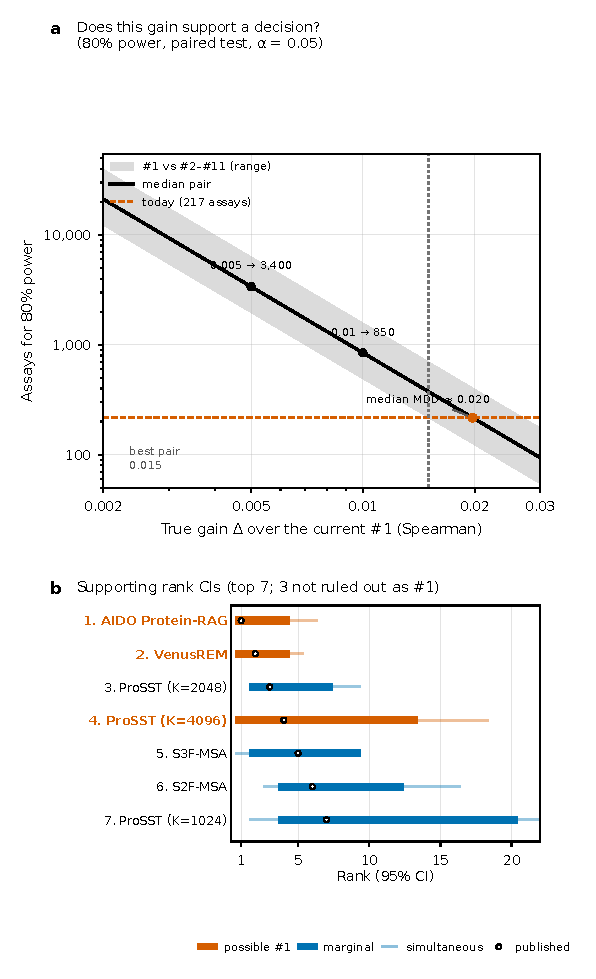
\includegraphics[width=\columnwidth]{../results/figures/headline.pdf}
\caption{\textbf{(a)} 95\% intervals for the rank of the ProteinGym aggregate, top 20 of \nModels{} models. Thick:
marginal (single-step max-$t$); thin: simultaneous (step-down). Orange: the 95\% best-model set. Dashed lines: the
only adjacent pairs that differ significantly (Holm). \topFour{} is a possible \#1 while \topThree{} is not: \#3 is
significantly below \topTwo{}, and \#4's paired standard errors are larger. \textbf{(b)} Assays needed for an
80\%-power test of a true gain $\Delta$ over the current \#1; the band spans the paired variances of \#1 against
each of the next ten models. Generated by \texttt{pgnoise figure}.}
\label{fig:headline}
\end{figure}

\begin{table}[t]
\centering\scriptsize
\caption{Coverage simulation: worst-model coverage of the true rank (nominal 0.95), range of joint coverage over
the five scenarios, and mean width of the top-10 intervals (calibrated scenario, ranks).}
\label{tab:sim}
\setlength{\tabcolsep}{3pt}
\begin{tabular}{@{}lccccccc@{}}
\toprule
Method & Calib. & Gauss. & Ties & Near & Sep. & Joint & Width \\
\midrule
Bootstrap percentile & \covPctCal & \covPctGauss & \covPctTies & \covPctNear & \covPctSep & \jointPctMin--\jointPctMax & \widthPct \\
Marginal, single-step & \covMargSSCal & \covMargSSGauss & \covMargSSTies & \covMargSSNear & \covMargSSSep & \jointMargSSMin--\jointMargSSMax & \widthMargSS \\
Marginal, step-down & \covMargSDCal & \covMargSDGauss & \covMargSDTies & \covMargSDNear & \covMargSDSep & \jointMargSDMin--\jointMargSDMax & \widthMargSD \\
Marginal, bootstrap-$t$ & \covMargSDtCal & \covMargSDtGauss & \covMargSDtTies & \covMargSDtNear & \covMargSDtSep & \jointMargSDtMin--\jointMargSDtMax & \widthMargSDt \\
Simultaneous, step-down & \covSimSDCal & \covSimSDGauss & \covSimSDTies & \covSimSDNear & \covSimSDSep & \jointSimSDMin--\jointSimSDMax & \widthSimSD \\
\bottomrule
\end{tabular}
\end{table}

\section{Results}
\textbf{The intervals are valid (Table~\ref{tab:sim}).} Marginal single-step and simultaneous step-down intervals
keep worst-model coverage at or above \covMargSSTies{} in every scenario. The price is width: the top-10 intervals
span \widthMargSS{} and \widthSimSD{} ranks on average, against \widthPct{} for the percentile interval. The percentile interval drops to \covPctTies{} for exactly tied
models. Marginal step-down under-covers under exact ties (\covMargSDTies{}; \covMargSDtTies{} when studentised), so
we do not use it for headline numbers. The best-model set contains a single true \#1 in at least \bestSingleMin\% of
runs. With a five-way tie at \#1 it contains each tied model \bestTiesEach\% and all five \bestTiesAll\% of the
time, compared with \naiveTiesAll\% for reading ProteinGym's error bars as ``within 1.96\,SE of \#1''.

\textbf{Ranks are uncertain (Fig.~\ref{fig:headline}a).} \topOne{} and \topTwo{} differ by \gapOneTwo{}, and each is
\#1 in about half of the bootstrap replicates (\pRankOneTop\% and \pRankOneSecond\%). The 95\% best-model set is
\bestSet{} (the naive reading gives \naiveBestSet{}). Only \nNeighbourSig{} of 19 adjacent pairs in the top 20
differ significantly (\sigPairA{}, $z=\zSigA$; \sigPairB{}, $z=\zSigB$), with or without Holm's correction. The
marginal interval for \#4 is ranks \margFourLo--\margFourHi{} and for \#10 \margTenLo--\margTenHi{}; the simultaneous
intervals extend to \simFourHi{} and \simTenHi{}. The gap between \#1 and \#3 is \gapOneThree{}
(SE \seOneThree, $z=\zOneThree$).

\textbf{The benchmark is underpowered at the top (Fig.~\ref{fig:headline}b).} With 80\% power the benchmark detects a
gain of about \mddMed{} over \#1 (\mddMin--\mddMax{} across the ten pairs). Detecting 0.01 needs about \unitsTenMed{}
units (\unitsTenMin--\unitsTenMax), or about \assaysTenMed{} assays, \timesTenMed$\times$ today; 0.005 needs about
\unitsFiveMed{} units (\unitsFiveMin--\unitsFiveMax), or \assaysFiveMed{} assays, \timesFiveMed$\times$ today.
Resampling agrees with the formula to within \powerSimGap{} in power, and the test's size is \sizeToday\% at today's
size and \sizeQuarter\% at a quarter of it. These figures are for one pairwise comparison; claiming a new \#1 against
every other model needs a multiplicity correction and more assays still.

\textbf{The top depends on the metric and the aggregation.} With \robBoot{} replicates per leaderboard: under Spearman,
AUC and MCC with any of four mean-based aggregations (ProteinGym's, function-group mean, protein-weighted, flat), the
possible-\#1 set stays within \robPossibleSSA{}; only the name in the \#1 slot changes (\robFgmLeader{} leads under
the function-group mean). Dropping the \logoFlipGroups{} assays makes \logoFlipLeader{} \#1. NDCG ranks
different models: \ndcgLeader{} is \#1, only \ndcgOverlap{} of the published top 10 stay in its top 10 (Kendall
$\tau=\ndcgTauMin$--$\ndcgTauMax$) and \ndcgBestMin--\ndcgBestMax{} models are possible \#1s. Top-$K$ recall leaves
\topkBestMin--\topkBestMax{} possible \#1s, and the median Spearman \medianBest{}. This echoes the general point that
aggregate leaderboards are sensitive to seemingly minor design choices~\cite{dehghani2021benchmark,zhang2024inherent}.

\textbf{Unequal assay coverage biases the ranking.} Protriever (\#\protRank) is scored on \protScored{} of \nAssays{}
assays, and it is the only incomplete model. Its \protMissing{} missing assays (\protMissAct{} Activity,
\protMissExp{} Expression, \protMissOrg{} OrganismalFitness, \protMissStab{} Stability) are harder for every other
model (mean Spearman \othersOnMissing{} against \othersOnCommon{}), so skipping them flatters it. On the
\nCommonAssays{} common assays it falls to \#\protRankCommon{} and \topOnCommon{} becomes \#1.

\textbf{Per-assay inputs replicate.} Re-scoring five small assays (one per function group) with ESM-2 8M--650M
\cite{lin2023evolutionary} on CPU, using ProteinGym's masked-marginal scoring~\cite{meier2021language}, reproduces
\esmExact/\esmCompared{} published Spearman values at 3\,dp (maximum difference \esmMaxDiff; \esmMaxDiffPG{} against
ProteinGym's own per-mutant scores) in \esmMinutes{} minutes. Scoring choices are as large as leaderboard gaps:
wild-type marginals move Spearman by up to \esmWtMax{} (median \esmWtMed), and pooling double mutants raises TCRG1
(650M) from \esmTcrgSingles{} on singles to \esmTcrgPooled. Within-assay mutant-bootstrap SEs are
\esmSeMin--\esmSeMax{}, and \esmStepsNeg{} of \esmSteps{} steps up in model size lower Spearman (\esmStepsNegSig{}
significantly). The rank uncertainty above therefore comes from which proteins are sampled, not from irreproducible
scores.

\section{Limitations}
\begin{itemize}
\item \textbf{Sampling model.} Proteins are treated as exchangeable draws within function groups. ProteinGym's
assays are curated, not sampled, so the intervals describe re-curation of similar proteins, not a different
curation policy.
\item \textbf{Unmodelled noise.} Mutant-level measurement noise, scoring choices and training randomness are not
propagated, so the intervals understate total uncertainty. Per-assay scores are rounded to 3\,dp.
\item \textbf{Small strata.} Binding has \unitsBinding{} units and Expression \unitsExpression; bootstrap critical
values are approximate there, which shows as the mildly liberal test size and the step-down under-coverage above.
\item \textbf{Conservative intervals.} Single-step intervals over-cover (mean coverage at least \meanCovMargSSMin{}
against 0.95), so the widths are an upper end.
\item \textbf{Power assumptions.} A new model is assumed to correlate with \#1 as today's challengers do, and new
assays to resemble current ones.
\item \textbf{Scope.} Protriever's missing block looks like a processing gap but is unconfirmed. The ESM-2 check
covers five short assays up to 650M parameters and does not exercise long-sequence windowing. This note is not peer
reviewed, and the novelty statement rests on a literature search of 6 October 2026.
\end{itemize}

\section{Proposed change for ProteinGym}
\texttt{performance\_DMS\_benchmarks.py} already draws \nBoot{} stratified bootstrap replicates for its error bars.
From the same replicates, at a cost of seconds and with no new data, it could: (1)~add to the leaderboard a
marginal 95\% rank interval, a simultaneous 95\% rank interval and a ``possible \#1'' flag (the 95\% best-model
set); (2)~rank models that skip assays on the common subset, or show their coverage next to their rank; and
(3)~state the minimum detectable difference (about \mddMed{} today) on the leaderboard page, so that new models are
not reported as state of the art on smaller differences. \texttt{pgnoise} implements all three and could be offered
as a pull request.

{\footnotesize
\bibliographystyle{abbrvnat}
\bibliography{refs}}

\end{document}
